\chapter{Exercise 1}

This task was done using Python with Numpy and SciPy.
The image manipulation library Pillow was also used indirectly by SciPy,
but only to load images into NumPy matrices and to save matrices to images.

\begin{lstlisting}[language=Python, caption=Utility functions]
def transform(matrix, fun):
    """
    applies fun(px) to every px in the 2d matrix
    """
    return np.asarray(map(lambda row: map(lambda px: fun(px), row), matrix))


def minmax_2d(matrix):
    """
    returns the minimum and maximum value of a 2d matrix
    """
    return map(lambda f: f(f(matrix, key=lambda x: f(x))), (min, max))


def random_matrix(w, h, n):
    """
    :returns a w*h matrix with random integers in the range [0, n>
    """
    return np.random.randint(n, size=(h, w))
\end{lstlisting}



\clearpage
\section*{Task 3 - Basic Image Manipulation}

\begin{lstlisting}[language=Python, label=flatfield, caption=Flatfield image correction]
def normalize_intensity(matrix):
    """
    normalizes the intensity values of the input matrix
    from the [0, 255] integer range to the [0, 1] floating point range
    """
    return transform(matrix, lambda px: px / 255)


def correct_with_flatfield(a, b):
    """
    :returns a new matrix with the quotients of each value in the matrices a and b
    """
    corrected = np.copy(a)
    for y, (a_row, b_row) in enumerate(zip(a, b)):
        for x, (a_px, b_px) in enumerate(zip(a_row, b_row)):
            corrected[y][x] = a_px / b_px

    return corrected
\end{lstlisting}

\begin{figure}[h!]
    \centering
    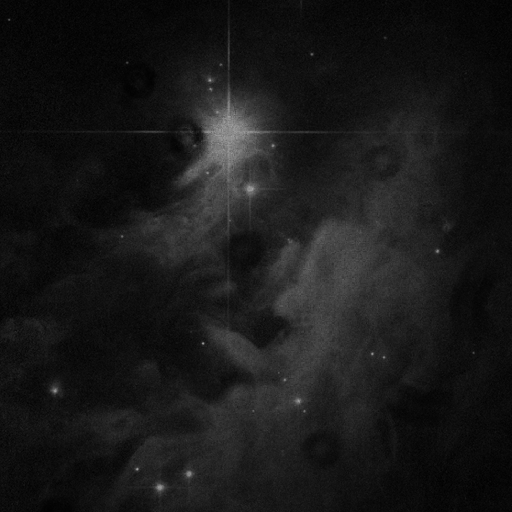
\includegraphics[width=5cm]{../LAB1/img/disturbed_potw1144a.png}
    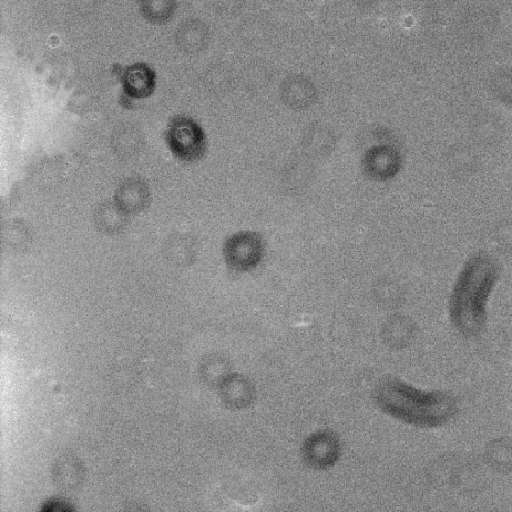
\includegraphics[width=5cm]{../LAB1/img/flatfieldimage.png}
    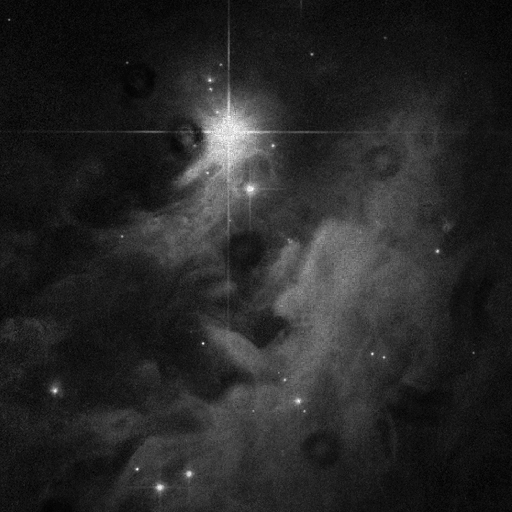
\includegraphics[width=5cm]{../LAB1/output/disturbed_potw1144a.png}
    \caption{From the left: original, flat-field image, corrected}
\end{figure}


\subsection*{2}
Flat-field correction is done by scaling with the intensity value of the pixel
in the image with the corresponding in the flat-field image.
The recorded value of an area is a function of the intensity of the region that is pictured,
and the distortion on the lens.
Using another method, like subtraction, would not give the desired effect.
E.g. if you took a pitch black picture with, subtracting the flat-field would yield invalid, negative values.
Using division, the result would be an unchanged picture, which in this case would be the correct result.



\clearpage
\section*{Task 4 - Point Processing}

Gamma correction is done by exponentially scaling every pixel intensity (range [0, 1]) in the image with the gamma factor.
\begin{lstlisting}[language=Python, label=gamma_correction, caption=Gamma correction]
def gamma_correct(matrix, gamma=1.0):
    """
    applies the gamma correction function (px)^(gamma) to the matrix
    """
    return transform(matrix, lambda px: int(255 * ((px / 255)**gamma)))
\end{lstlisting}

For the second part of the task, we need to find the maximum and minimum intensity level of the image.
Using these values, we can again apply a function to every pixel in the image,
which first skews every value towards 0 then scales them so that the largest value becomes 255.

\begin{lstlisting}[language=Python, label=input_range, caption=Input range stretching]
def stretch_range(matrix):
    """
    stretches the range of matrix to [0, 255]
    """
    lo, hi = minmax_2d(matrix)
    return transform(matrix, lambda px: int((px - lo) / ((hi - lo) / 255)))
\end{lstlisting}

\begin{figure}[h!]
    \centering
    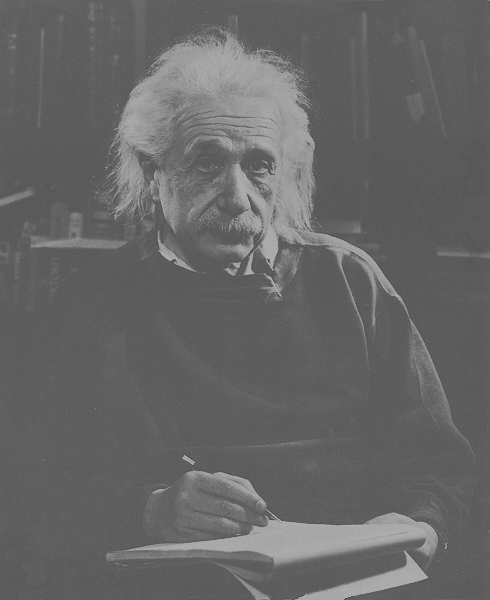
\includegraphics[width=5cm]{../LAB1/img/einstein_lowcontrast.png}
    \includegraphics[width=5cm]{../LAB1/output/gamma_einstein_lowcontrast.png}
    \includegraphics[width=5cm]{../LAB1/output/stretched_gamma_einstein_lowcontrast.png}
    \caption{Left: Original einstein\_lowcontrast.png, middle: gamma corrected, right: input range stretched then gamma corrected.}
\end{figure}



\clearpage
\subsection*{Histogram equalization}

To create a histogram we iterate over the pixels and count the occurrences.
To normalize we need the sum of counts (aka. the picture size), which we divide every count by.
Finally a helper function takes the normalized histogram and returns a cummulative distribution function representing the histogram.

\begin{lstlisting}[language=Python, label=input_range, caption=Input range stretching]
def create_histogram(matrix):
    """
    counts the occurences of each value in the matrix
    """
    histogram = defaultdict(int)
    for row in matrix:
        for px in row:
            histogram[px] += 1

    return histogram


def normalize_histogram(histogram):
    """
    normalizes the values in a histogram, aka. creates a distribution histogram
    """
    normalized = dict()
    total = sum(histogram.values())
    for key, value in histogram.iteritems():
        normalized[key] = value / total

    return normalized


def create_cdf(normalized_histogram):
    """
    :returns a cummulative distribution function that can be called with a value parameter
    """
    return lambda i: sum(normalized_histogram[j] for j in [v for v in normalized_histogram.keys() if v <= i])
\end{lstlisting}

\newpage
\begin{figure}[h!]
    \centering
 \begin{verbatim}
 [[2 2 6 6]     [[ 0.25    0.25    0.9375  0.9375]
  [3 3 1 4]      [ 0.375   0.375   0.125   0.6875]
  [0 6 5 4]      [ 0.0625  0.9375  0.75    0.6875]
  [4 4 4 7]]     [ 0.6875  0.6875  0.6875  1.    ]]
 \end{verbatim}
 \caption{Left: Randomly generated matrix.\\
 Right: The same matrix after using the cummulative distribution function on every value.}
\end{figure}

\begin{figure}[h!]
    \centering
    \includegraphics[width=5cm]{../LAB1/output/cdf_einstein_lowcontrast.png}
    \caption{cdf applied to the Einstein picture.}
\end{figure}


\clearpage
\section*{Task 5 - Noise}

\subsection*{1 - Salt \& Pepper noise}

\begin{lstlisting}[language=Python, label=salt-and-pepper, caption=Salt \& pepper noise]
def salt_and_pepper_noise(matrix, density):
    """
    :returns the matrix with some noise randomly added.
    Each noisy pixel will randomly be either black or white.
    The amount of noise increases with the parameter density
    """
    return transform(matrix, lambda px: np.random.randint(2) if np.random.random() < density else px)
\end{lstlisting}


\begin{figure}[h!]
    \centering
    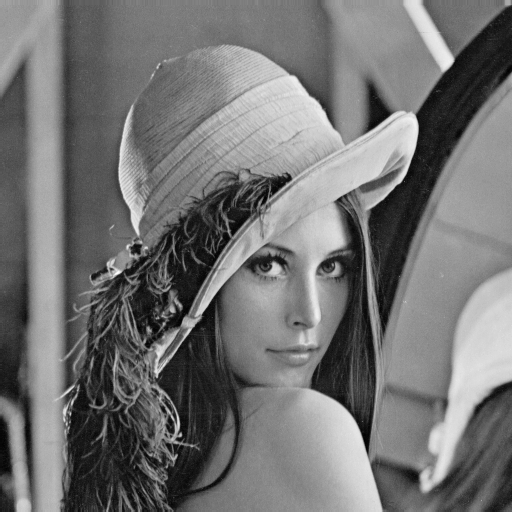
\includegraphics[width=5cm]{../LAB1/img/lena.png}
    \includegraphics[width=5cm]{../LAB1/output/noisy_0_1.png} \\
    \includegraphics[width=5cm]{../LAB1/output/noisy_0_3.png}
    \includegraphics[width=5cm]{../LAB1/output/noisy_0_8.png}
    \caption{Original, density = 0.1,\\ density = 0.3, density = 0.8}
\end{figure}

Other types of noise include gaussian, shot, uniform, film grain and anisotropic.



\clearpage
\section*{Task 6 - Aliasing}

We observe aliasing, specifically a \textit{moiré pattern}.

\begin{lstlisting}[language=Python, label=aliasing, caption=Aliasing function]
def alias(matrix, n):
    """
    Downscales the matrix by removing every row and column except every nth.
    """
    return np.asarray(
        [[px for x, px in enumerate(row) if x % n == 0] for y, row in enumerate(matrix) if y % n == 0]
    )
\end{lstlisting}

\begin{figure}[h!]
    \centering
    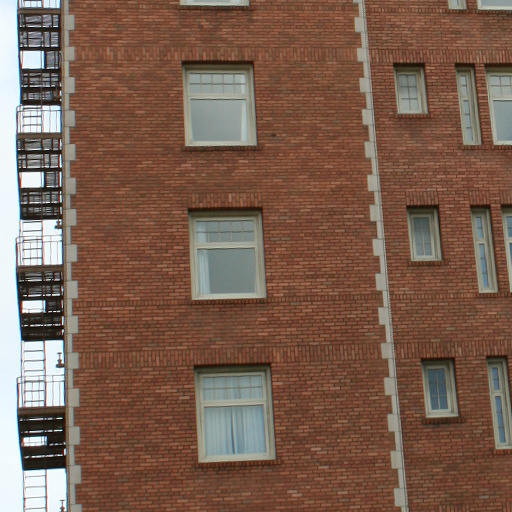
\includegraphics[width=5cm]{../LAB1/img/bricks.png}
    \includegraphics[width=5cm]{../LAB1/output/brick_down_2x.png} \\
    \includegraphics[width=5cm]{../LAB1/output/brick_down_3x.png}
    \includegraphics[width=5cm]{../LAB1/output/brick_down_4x.png}
    \caption{Original, factor = 2,\\ factor = 3, factor = 4}
\end{figure}


\begin{figure}[h!]
    \centering
    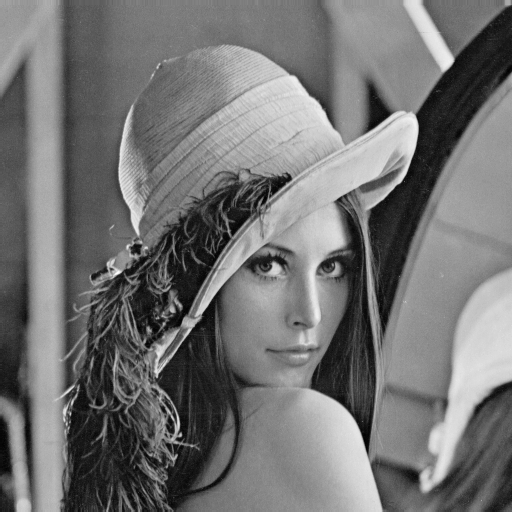
\includegraphics[width=5cm]{../LAB1/img/lena.png}
    \includegraphics[width=5cm]{../LAB1/output/lena_down_2x.png} \\
    \includegraphics[width=5cm]{../LAB1/output/lena_down_3x.png}
    \includegraphics[width=5cm]{../LAB1/output/lena_down_4x.png}
    \caption{Original, factor = 2,\\ factor = 3, factor = 4}
\end{figure}
